%%%%%%%%%%%%%%%%%%%%%%%%%5
%% abtex2-modelo-trabalho-academico.tex, v<VERSION> laurocesar
%% Copyright 2012-<COPYRIGHT_YEAR> by abnTeX2 group at http://www.abntex.net.br/ 
%%
%% This work may be distributed and/or modified under the
%% conditions of the LaTeX Project Public License, either version 1.3
%% of this license or (at your option) any later version.
%% The latest version of this license is in
%%   http://www.latex-project.org/lppl.txt
%% and version 1.3 or later is part of all distributions of LaTeX
%% version 2005/12/01 or later.
%%
%% This work has the LPPL maintenance status `maintained'.
%% 
%% The Current Maintainer of this work is the abnTeX2 team, led
%% by Lauro César Araujo. Further information are available on 
%% http://www.abntex.net.br/
%%
%% This work consists of the files abntex2-modelo-trabalho-academico.tex,
%% abntex2-modelo-include-comandos and abntex2-modelo-references.bib
%%

% ------------------------------------------------------------------------
% ------------------------------------------------------------------------
% abnTeX2: Modelo de Trabalho Academico (tese de doutorado, dissertacao de
% mestrado e trabalhos monograficos em geral) em conformidade com 
% ABNT NBR 14724:2011: Informacao e documentacao - Trabalhos academicos -
% Apresentacao
% ------------------------------------------------------------------------
% ------------------------------------------------------------------------

\documentclass[
	% -- opções da classe memoir --
	12pt,				% tamanho da fonte
  openright,			% capítulos começam em pág ímpar (insere página vazia caso preciso)
	twoside,			% para impressão em recto e verso. Oposto a oneside
	a4paper,			% tamanho do papel. 
	% -- opções da classe abntex2 --
	%chapter=TITLE,		% títulos de capítulos convertidos em letras maiúsculas
	%section=TITLE,		% títulos de seções convertidos em letras maiúsculas
	%subsection=TITLE,	% títulos de subseções convertidos em letras maiúsculas
	%subsubsection=TITLE,% títulos de subsubseções convertidos em letras maiúsculas
	% -- opções do pacote babel --
	english,			% idioma adicional para hifenização
	french,				% idioma adicional para hifenização
	spanish,			% idioma adicional para hifenização
	brazil				% o último idioma é o principal do documento
	]{abntex2}

% ---
% Pacotes básicos 
% ---
\usepackage{lmodern}			% Usa a fonte Latin Modern			
\usepackage[T1]{fontenc}		% Selecao de codigos de fonte.
\usepackage[utf8]{inputenc}		% Codificacao do documento (conversão automática dos acentos)
\usepackage{lastpage}			% Usado pela Ficha catalográfica
\usepackage{indentfirst}		% Indenta o primeiro parágrafo de cada seção.
\usepackage{color}				% Controle das cores
\usepackage{graphicx}			% Inclusão de gráficos
\usepackage{microtype} 			% para melhorias de justificação
% ---
		
% ---
% Pacotes adicionais, usados apenas no âmbito do Modelo Canônico do abnteX2
% ---
\usepackage{lipsum}				% para geração de dummy text
% ---

% ---
% Pacotes de citações
% ---
\usepackage[brazilian,hyperpageref]{backref}	 % Paginas com as citações na bibl
\usepackage[alf]{abntex2cite}	% Citações padrão ABNT

% --- 
% CONFIGURAÇÕES DE PACOTES
% --- 

% ---
% Configurações do pacote backref
% Usado sem a opção hyperpageref de backref
\renewcommand{\backrefpagesname}{Citado na(s) página(s):~}
% Texto padrão antes do número das páginas
\renewcommand{\backref}{}
% Define os textos da citação
\renewcommand*{\backrefalt}[4]{
	\ifcase #1 %
		Nenhuma citação no texto.%
	\or
		Citado na página #2.%
	\else
		Citado #1 vezes nas páginas #2.%
	\fi}%
% ---

% ---
% Informações de dados para CAPA e FOLHA DE ROSTO
% ---
\titulo{Apresentação do Limarka}
\autor{Eduardo de Santana Medeiros Alexandre}
\data{2016}
\local{João Pessoa}
\orientador{Fulano de tal}
\coorientador{}
\instituicao{%
  Universidade Federal da Paraíba
  \par
  Computação
}
\tipotrabalho{Monografia}

% O preambulo deve conter o tipo do trabalho, o objetivo (propósito), 
% o nome da instituição e a área de concentração.
% Esse texto irá compor a Folha de Rosto e Folha de Aprovação.
\preambulo{
% Propósito gerado automaticamente.
Monografia apresentada ao Curso de Computação da Universidade Federal da Paraíba, como requisito parcial para obtenção do grau de Bacharel em Computação.
\newline\textbf{Área de concentração}: Computação.
}%% fim do preambulo




% ---
% Configurações de aparência do PDF final

% alterando o aspecto da cor azul
\definecolor{blue}{RGB}{41,5,195}

% informações do PDF
\makeatletter
\hypersetup{
     	%pagebackref=true,
		pdftitle={\@title}, 
		pdfauthor={\@author},
    	pdfsubject={\imprimirpreambulo},
	    pdfcreator={LaTeX with abnTeX2 and Limarka},
		pdfkeywords={abnt}{latex}{abntex}{abntex2}{trabalho acadêmico}, 
		colorlinks=true,       		% false: boxed links; true: colored links
    	linkcolor=blue,          	% color of internal links
    	citecolor=blue,        		% color of links to bibliography
    	filecolor=magenta,      		% color of file links
		urlcolor=blue,
		bookmarksdepth=4
}
\makeatother
% --- 

% --- 
% Espaçamentos entre linhas e parágrafos 
% --- 

% O tamanho do parágrafo é dado por:
\setlength{\parindent}{1.3cm}

% Controle do espaçamento entre um parágrafo e outro:
\setlength{\parskip}{0.2cm}  % tente também \onelineskip

% ---
% compila o indice
% ---
\makeindex
% ---

%---
% CONFIGURAÇÕES EXTRA DO LIMARKA
%---

% Configura citações de pandoc para 4cm à esquerda (utiliza o ambiente quote)
\renewenvironment{quote}
  {\small\list{}{\rightmargin=0.1cm \leftmargin=4cm}%
   \item\relax}
  {\endlist}

% Para incluir páginas PDF (ficha catalografica e folha de aprovação)
\usepackage[dvipsnames]{xcolor} % http://tex.stackexchange.com/questions/124636/package-xcolor-error-undefined-colors-maroon-royal-blue-when-master-has-pdf
\usepackage{pdfpages}
\usepackage{longtable} % para as tabelas
%\usepackage{floatrow}
%\floatsetup[figure]{capposition=top}


%%
%% Esse modelo é responsável pela impressão dos seguintes elementos:
%% Capa, Folha de rosto e Ficha catalográfica.


% ----
% Início do documento
% ----
\begin{document}

% Seleciona o idioma do documento (conforme pacotes do babel)
%\selectlanguage{english}
\selectlanguage{brazil}

% Retira espaço extra obsoleto entre as frases.
\frenchspacing 

% ----------------------------------------------------------
% ELEMENTOS PRÉ-TEXTUAIS
% ----------------------------------------------------------
% \pretextual

% ---
% Capa
% ---
\imprimircapa
% ---

% ----------------------------------------------------------
% ELEMENTOS PRÉ-TEXTUAIS
% ----------------------------------------------------------
% \pretextual

% ---
% Folha de rosto: sempre será impressa
% ---
\imprimirfolhaderosto
% ---
% Sem ficha catalográfica
% ---
% ---


% ---
% ERRATA: Sem errata
% ---


% ---
% Sem Folha de aprovação
% ---
% ---

% ---
% Dedicatória
% ---
% ---
% Agradecimentos
% ---
% ---
% Epígrafe
% ---
% ---

% ---
% Resumo na língua vernácula (obrigatório)
% ---


% ---
% Resumo em língua estrangeira (obrigatório)
% ---



% ---

% ---
% Lista de ilustrações (opcional): não utilizando.
% ---
% ---
% Lista de tabelas (opcional): não utilizando
% ---

% ---
% Lista de abreviaturas e siglas (opcional)
% ---
\begin{siglas}
  \item[ABNT] Associação Brasileira de Normas Técnicas
\end{siglas}
% ---

% ---
% Lista de símbolos (opcional): AUSENTE
% ---
% ---
% Sumário
% ---
\pdfbookmark[0]{\contentsname}{toc}
\tableofcontents*
\cleardoublepage
% ---


% ----------------------------------------------------------
% ELEMENTOS TEXTUAIS
% ----------------------------------------------------------
\textual

%%
%% Texto será incluído aqui
%%
\chapter{Introdução}\label{introduuxe7uxe3o}

\section{Sintaxe básica do
Markdown}\label{sintaxe-buxe1sica-do-markdown}

Mesmo que eu digite um texto quebrado em várias linhas, mesmo assim, ele
será apresentado como um único parágrafo.

Aqui é o inicia um novo parágrafo.

Formatação de palavras: \emph{itálico}, \textbf{negrito}.

Listas não ordenadas

\begin{itemize}
\tightlist
\item
  Objetivo 1;
\item
  Objetivo 2;
\item
  Objetivo 3.
\end{itemize}

Ou também:

\begin{itemize}
\tightlist
\item
  Objetivo 1;
\item
  Objetivo 2;
\item
  Objetivo 3.
\end{itemize}

Listas ordenadas com números

\begin{enumerate}
\def\labelenumi{\arabic{enumi}.}
\tightlist
\item
  Primeiro item da lista;
\item
  Segundo item da lista;
\item
  Terceiro item da lista.
\end{enumerate}

Listas ordenadas com letras

\begin{enumerate}
\def\labelenumi{\alph{enumi}.}
\tightlist
\item
  Primeiro item da lista;
\item
  Segundo item da lista;
\item
  Terceiro item da lista.
\end{enumerate}

Ou também:

\begin{enumerate}
\def\labelenumi{\alph{enumi})}
\tightlist
\item
  Primeiro item da lista;
\item
  Segundo item da lista;
\item
  Terceiro item da lista.
\end{enumerate}

Adoro várias frutas: banana, caju e morango.\footnote{Morango não é
  fruta.}

\chapter{Como inserir código Latex}\label{como-inserir-cuxf3digo-latex}

O código latex pode ser inserido ao longo do texto:

\begin{array}{c|c}
  1 & 2 \\ 
  \hline
  3 & 4
\end{array}

Inclusive dentro do parágrafo, como podemos ver: \sqrt{81}.

\chapter{Como inserir imagens}\label{como-inserir-imagens}

\begin{figure}[htbp]
\caption{\label{fig:passaro}Legenda da figura.}
\begin{center}
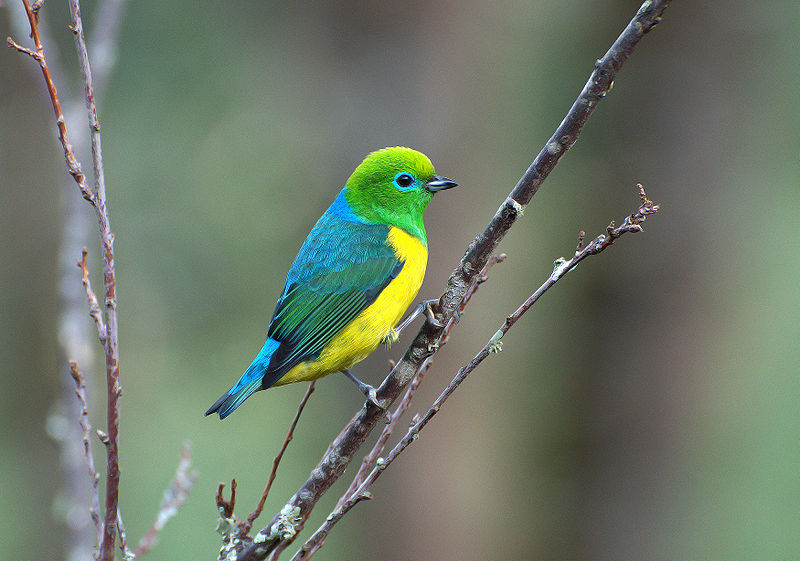
\includegraphics[width=0.5\textwidth]{imagens/passaro.jpg}
\end{center}
\legend{Fonte: Autor.}
\end{figure}

Como escolher o tamanho ideal? Esse foi o escolhido!

\begin{figure}[htbp]
\caption{\label{fig:passaro}Legenda da figura.}
\begin{center}
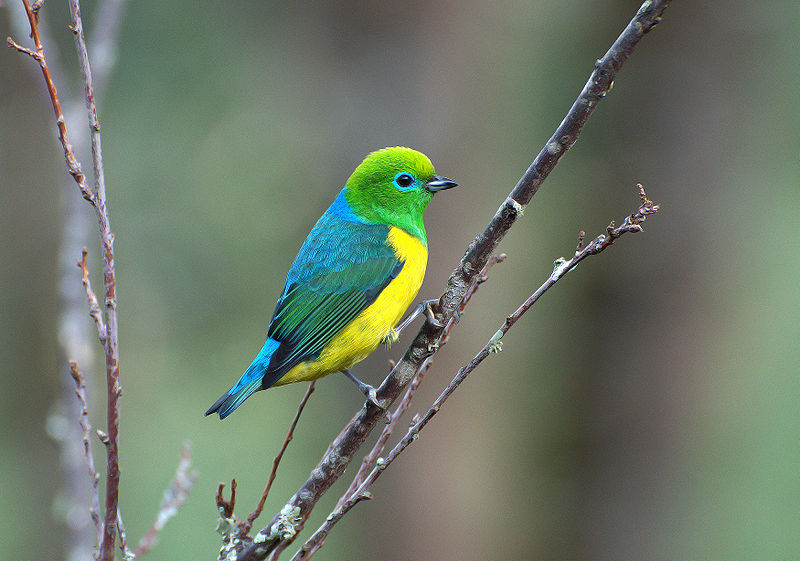
\includegraphics[width=0.4\textwidth]{imagens/passaro.jpg}
\end{center}
\legend{Fonte: Autor.}
\end{figure}

É possível verificar um pássaro (ver Figura \ref{fig:passaro}) com as
cores da bandeira do Brasil.

\chapter{Nova imagem}\label{nova-imagem}

\begin{figure}[htbp]
\caption{\label{fig:rex}Legenda da figura.}
\begin{center}
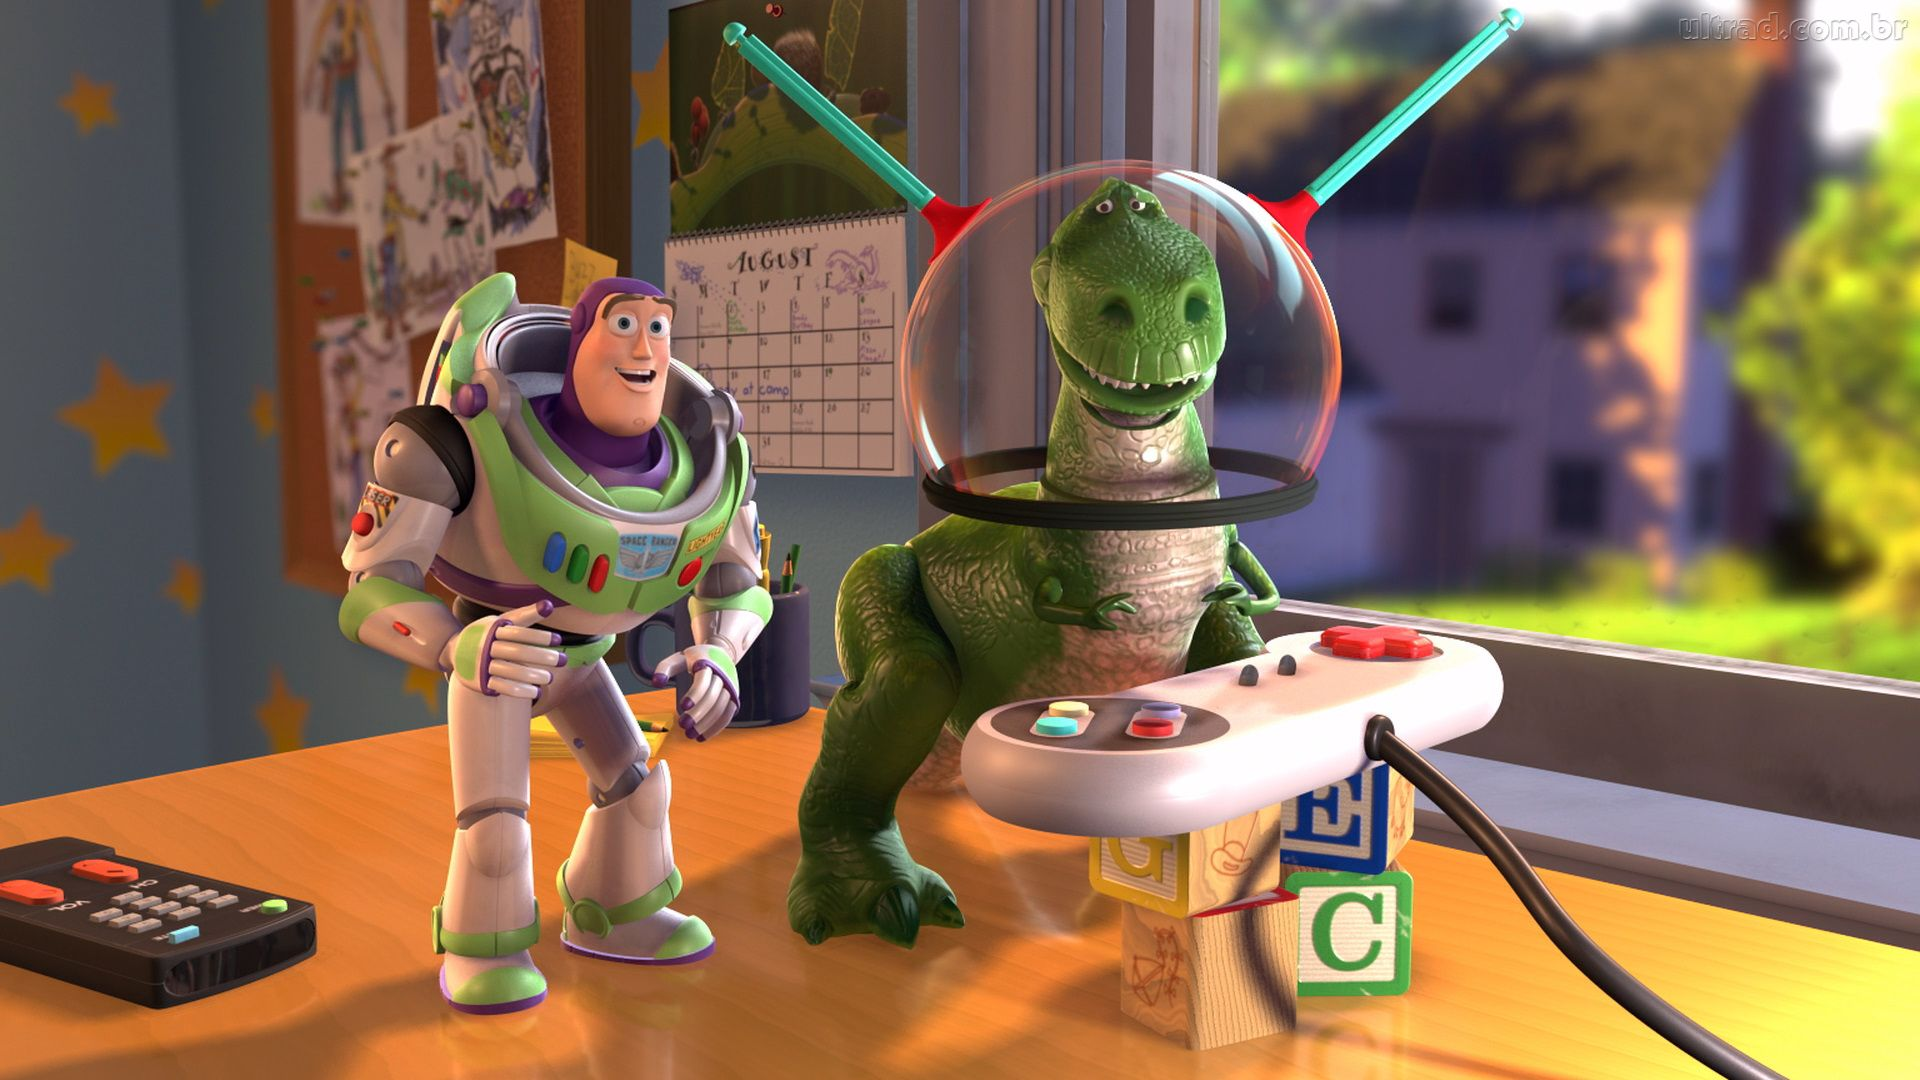
\includegraphics[width=0.6\textwidth]{imagens/Buzz-e-Rex-Jogando-Videogame-Toy-Story_1920x1080.jpg}
\end{center}
\legend{Fonte: Autor.}
\end{figure}
\begin{figure}[htbp]
\caption{\label{fig:rex}Legenda da figura.}
\begin{center}
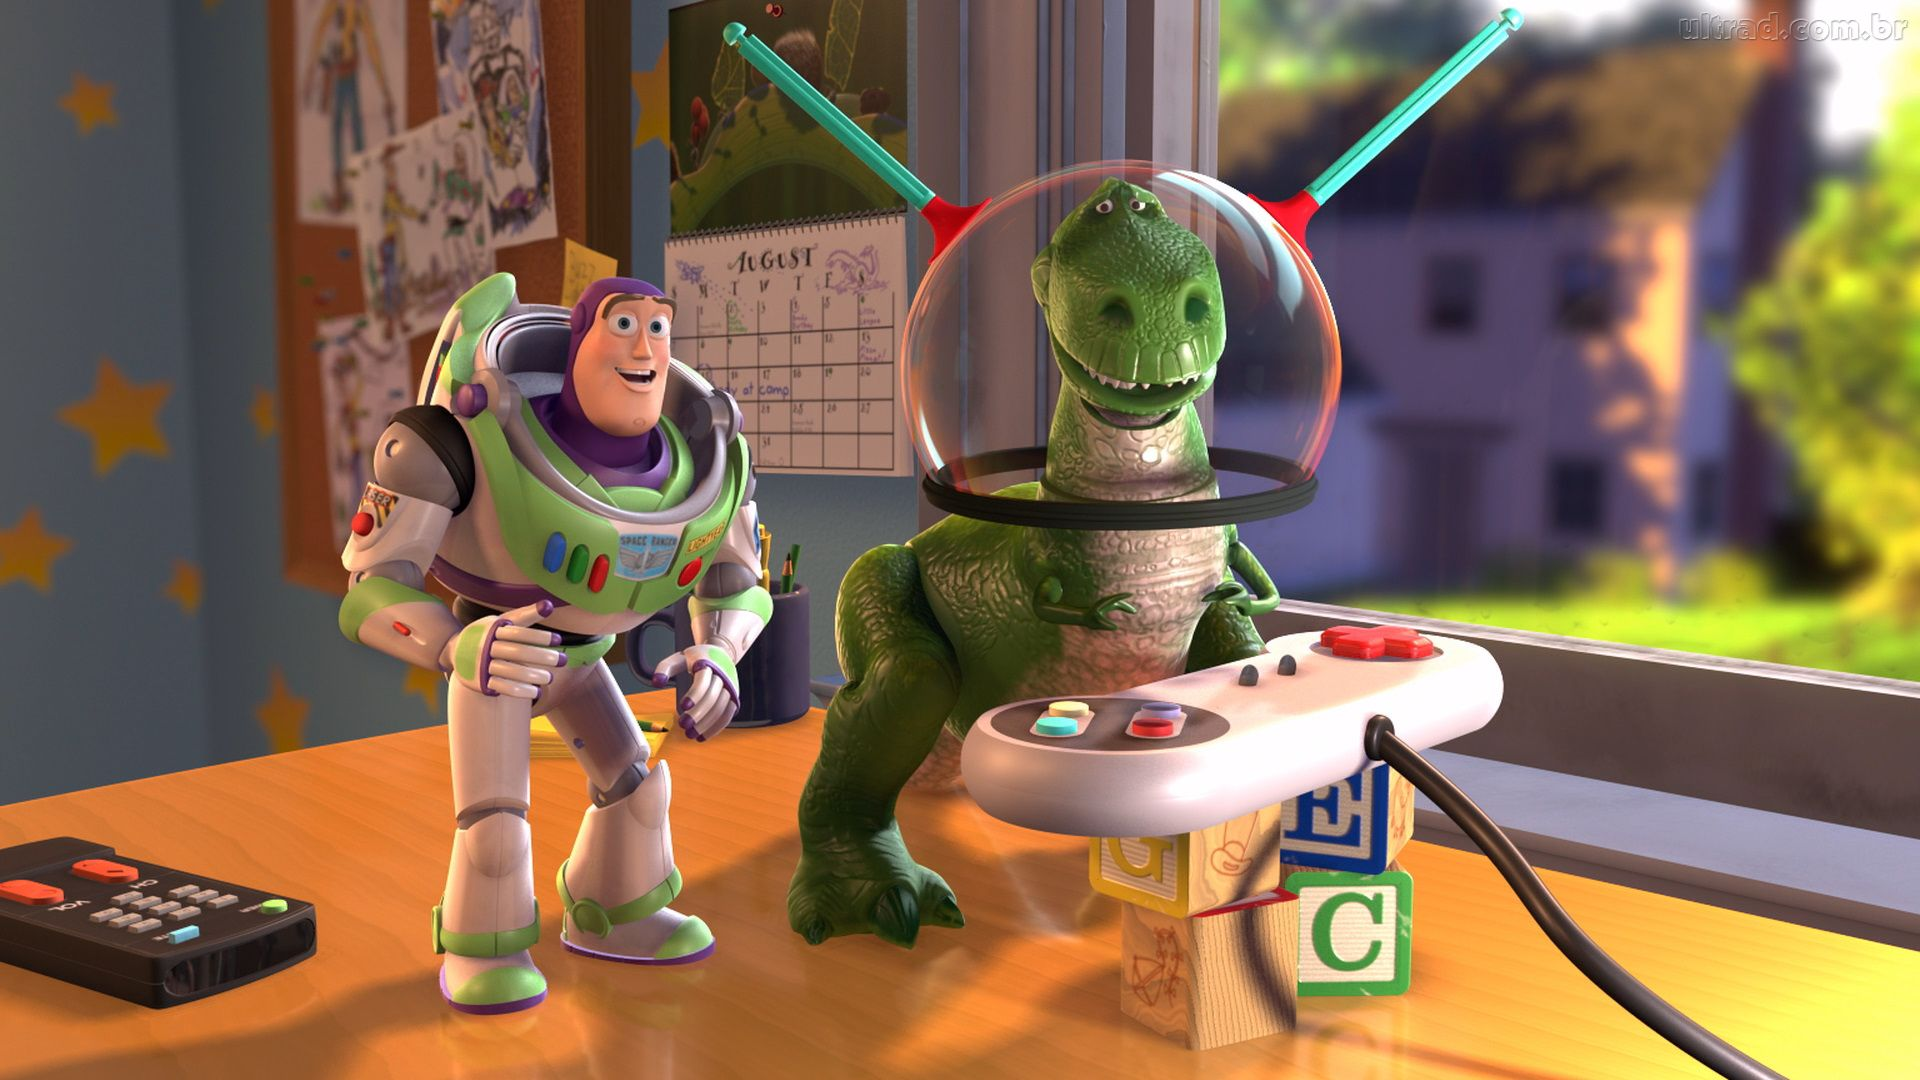
\includegraphics[width=0.7\textwidth]{imagens/Buzz-e-Rex-Jogando-Videogame-Toy-Story_1920x1080.jpg}
\end{center}
\legend{Fonte: Autor.}
\end{figure}

Dinossauro Buzz Figura \ref{fig:rex}.

\chapter{Inserindo tabelas}\label{cap:inserir-tabelas}

As tabelas são inseridas através de código latex.

Ver a documentação do abntex2 -- Manual do abntex, seção 6.5 Tabelas em
conformidade com padrões do IBGE.

\begin{table}[htb]
\ABNTEXfontereduzida
\caption[Legenda da tabela.]{Legenda da tabela.}
\label{tab:15560}
\begin{tabular}{p{2.6cm}|p{6.0cm}|p{2.25cm}|p{3.40cm}}
  %\hline
   \textbf{Nível de Investigação} & \textbf{Insumos}  & \textbf{Sistemas de Investigação}  & \textbf{Produtos}  \\
    \hline
    Meta-nível & Filosofia\index{filosofia} da Ciência  & Epistemologia &
    Paradigma  \\
    \hline
    Nível do objeto & Paradigmas do metanível e evidências do nível inferior &
    Ciência  & Teorias e modelos \\
    \hline
    Nível inferior & Modelos e métodos do nível do objeto e problemas do nível inferior & Prática & Solução de problemas  \\
   % \hline
\end{tabular}
\legend{Fonte: Autor.}
\end{table}
\begin{table}[htb]
\IBGEtab{%
  \caption{Legenda da tabela.}%
  \label{tab:15560}
}{%
  \begin{tabular}{ccc}
  \toprule
   Nome & Nascimento & Documento \\
  \midrule \midrule
   Maria da Silva & 11/11/1111 & 111.111.111-11 \\
  \midrule 
   João Souza & 11/11/2111 & 211.111.111-11 \\
  \midrule 
   Laura Vicuña & 05/04/1891 & 3111.111.111-11 \\
  \bottomrule
\end{tabular}%
}{%
  \fonte{Autor.}%
}
\end{table}

Percebemos que Maria da Silva é a mais nova de todos (ver Tabela
\ref{tab:15560}).

\chapter{Elaborando uma citação INDIRETA (preferível pois evita
acusações de
plágio)}\label{elaborando-uma-citauxe7uxe3o-indireta-preferuxedvel-pois-evita-acusauxe7uxf5es-de-pluxe1gio}

Os cursos não são ofertados pela UAB, mas pelas instituições associadas
à ela \cite{preti2005educaccao}.

\chapter{Configurando o Jabref para utilização com o
abntex2}\label{configurando-o-jabref-para-utilizauxe7uxe3o-com-o-abntex2}

Seguir as instruções em https://github.com/abntex/abntex2/wiki/JabRef

\chapter{Refências e citações diretas com o limarka e o Jabref
personalizado para o abntex2}\label{capitulo:citacoes}

\textbf{ABNT}: As citações diretas devem fornecer a página.

\section{Citação direta com até três
linhas}\label{secao:citacao-indireta}

``A Lesão da Substância Branca (LSB) é indicada como sendo a mais
frequente lesão cerebral em RN pré-termo e a termo''
\cite[p. 7]{almeida2013}.

\section{Citação direta com quatro ou mais
linhas}\label{secao:citacao-direta}

\begin{quote}
Evidencia-se a associação entre o tempo de gestação e o aumento do risco
para o desenvolvimento de doenças cardiovasculares e outros agravos
crônicos tanto em fases mais precoces da vida quanto em fases mais
tardias (vida adulta). A prematuridade ocorre frequentemente em
concomitância com o baixo peso, contribuindo para o desenvolvimento dos
mais variados impactos, a exemplo da hiperbilirrubinemia.
\cite[p. 7]{almeida2013}
\end{quote}

\chapter{Referenciando capítulos ou seções no
limarka}\label{cap:rotulos}

As referências são realizadas através de rótulos, similar as Figuras e
Tabelas. Os nomes dos rótulos são elaborados com prefixos para lembrar
que tipo de rótulo estamos nos referindo. Então \texttt{fig:passaro} é
um rótulo para uma figura (prefixo \texttt{fig:}). Os prefixos para
capítulos e seção costumam ser \texttt{cap} e \texttt{sec}, mas são
apenas sugestões.

Outro aspecto relevante é a sintaxe para DEFINIR rótulos em capítulos e
seções. Basta adicionar \texttt{\{\#cap:rotulo-do-capitulo\}} ou
\texttt{\{\#sec:rotulo-da-secao\}} após seus títulos.

\section{Exemplo de seção com rótulo}\label{sec:exemplo-de-rotulo}

Para saber como incluir rótulo em seções consulte Seção
\ref{sec:exemplo-de-rotulo}, ou o capítulo \ref{cap:rotulos}.

\chapter{Utilizando Anexos e
Apêndices}\label{utilizando-anexos-e-apuxeandices}

Os anexos e apêndices são digitados nos arquivos \texttt{anexos.md} e
\texttt{apendices.md} respectivamente. A sintaxe de edição é semelhante
ao do arquivo \texttt{trabalho-academico.md}. A diferença é que nesses
arquivos os capítulos tornam-se Anexos ou Apêndices.

Para utilização desses elementos é necessário \emph{habilitar} sua
utilização no arquivo \texttt{configuracao.pdf}.

\section{Referenciando anexos e
apêndices}\label{referenciando-anexos-e-apuxeandices}

O roteiro de entrevista encontra-se no Apêndice
\ref{apendice:entrevista}. E a questionário reutilizado em nossa
pesquisa encontra-se no Anexo \ref{anexo:questionario}.



% ----------------------------------------------------------
% ELEMENTOS PÓS-TEXTUAIS
% ----------------------------------------------------------
\postextual
% ----------------------------------------------------------

% ----------------------------------------------------------
% Início dos ELEMENTOS PÓS-TEXTUAIS
% ----------------------------------------------------------
\postextual
% ----------------------------------------------------------

% ----------------------------------------------------------
% Referências bibliográficas
% ----------------------------------------------------------
\bibliography{xxx-referencias}
% ----------------------------------------------------------
% Apêndices
% ----------------------------------------------------------
% 
% ---
% Inicia os apêndices
% ---
\begin{apendicesenv}

% Imprime uma página indicando o início dos apêndices
\partapendices

\chapter{Roteiro de Entrevista}\label{apendice:entrevista}

Texto do apêndice aqui. Este apêndice poderia representar um roteiro de
entrevista elaborado pelo pesquisador.

\lipsum[50]

\section{Roteiro}\label{roteiro}

Também é possível criar seções, incluir imagens, tabelas etc.

\lipsum[51]

\chapter{Segundo apêndice}\label{segundo-apuxeandice}

Para criar um novo apêndice, basta criar um novo capítulo!

\lipsum[55-57]

\end{apendicesenv}

% ----------------------------------------------------------
% Anexos
% ----------------------------------------------------------
\begin{anexosenv}
% Imprime uma página indicando o início dos anexos
\partanexos
\chapter{Primeiro anexo}\label{anexo:questionario}

\lipsum[30]

\chapter{Questionário da Pesquisa}\label{anexo:questionario}

Segue o questionário reutilizado em nossa pesquisa.

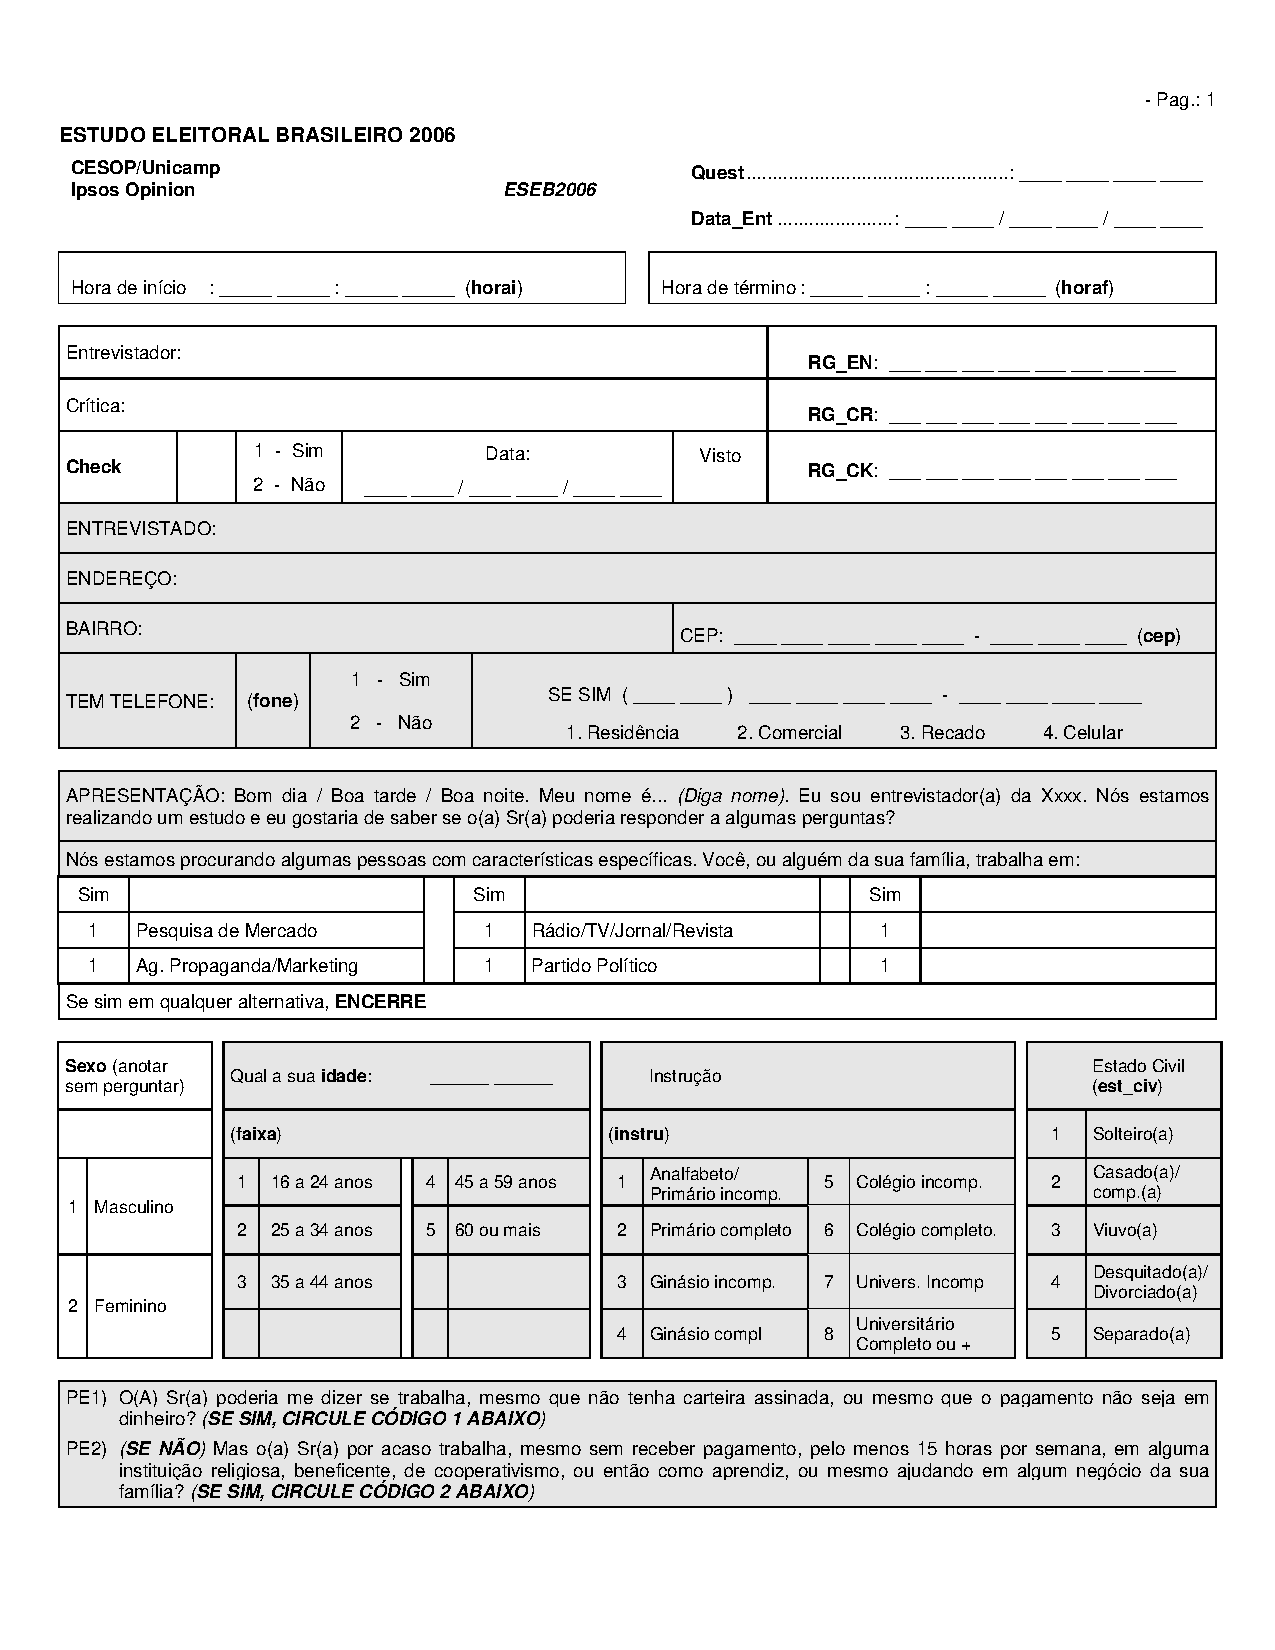
\includepdf[pages=-]{imagens/questionario_BRA_2006_Untrans_Portuguese.pdf}
\end{anexosenv}



\end{document}

